%
% $RCSfile: cybop_approach.tex,v $
%
% Copyright (C) 2002-2008. Christian Heller.
%
% Permission is granted to copy, distribute and/or modify this document
% under the terms of the GNU Free Documentation License, Version 1.1 or
% any later version published by the Free Software Foundation; with no
% Invariant Sections, with no Front-Cover Texts and with no Back-Cover
% Texts. A copy of the license is included in the section entitled
% "GNU Free Documentation License".
%
% http://www.cybop.net
% - Cybernetics Oriented Programming -
%
% http://www.resmedicinae.org
% - Information in Medicine -
%
% Version: $Revision: 1.1 $ $Date: 2008-08-19 20:41:06 $ $Author: christian $
% Authors: Christian Heller <christian.heller@tuxtax.de>
%

\paragraph{CYBOP}
\label{cybop_approach_heading}
\index{Cybernetics Oriented Programming Approach}
\index{CYBOP Approach}
\index{Cybernetics Oriented Language}
\index{CYBOL}
\index{Cybernetics Oriented Interpreter}
\index{CYBOI}
\index{Res Medicinae}

In CYBOP, all knowledge, that is states as well as logic, belongs to the
\emph{Statics} of a system. It is described by fixed structures. The processing
of knowledge at runtime, in order to control a system, is called \emph{Dynamics}.

\begin{figure}[ht]
    \begin{center}
        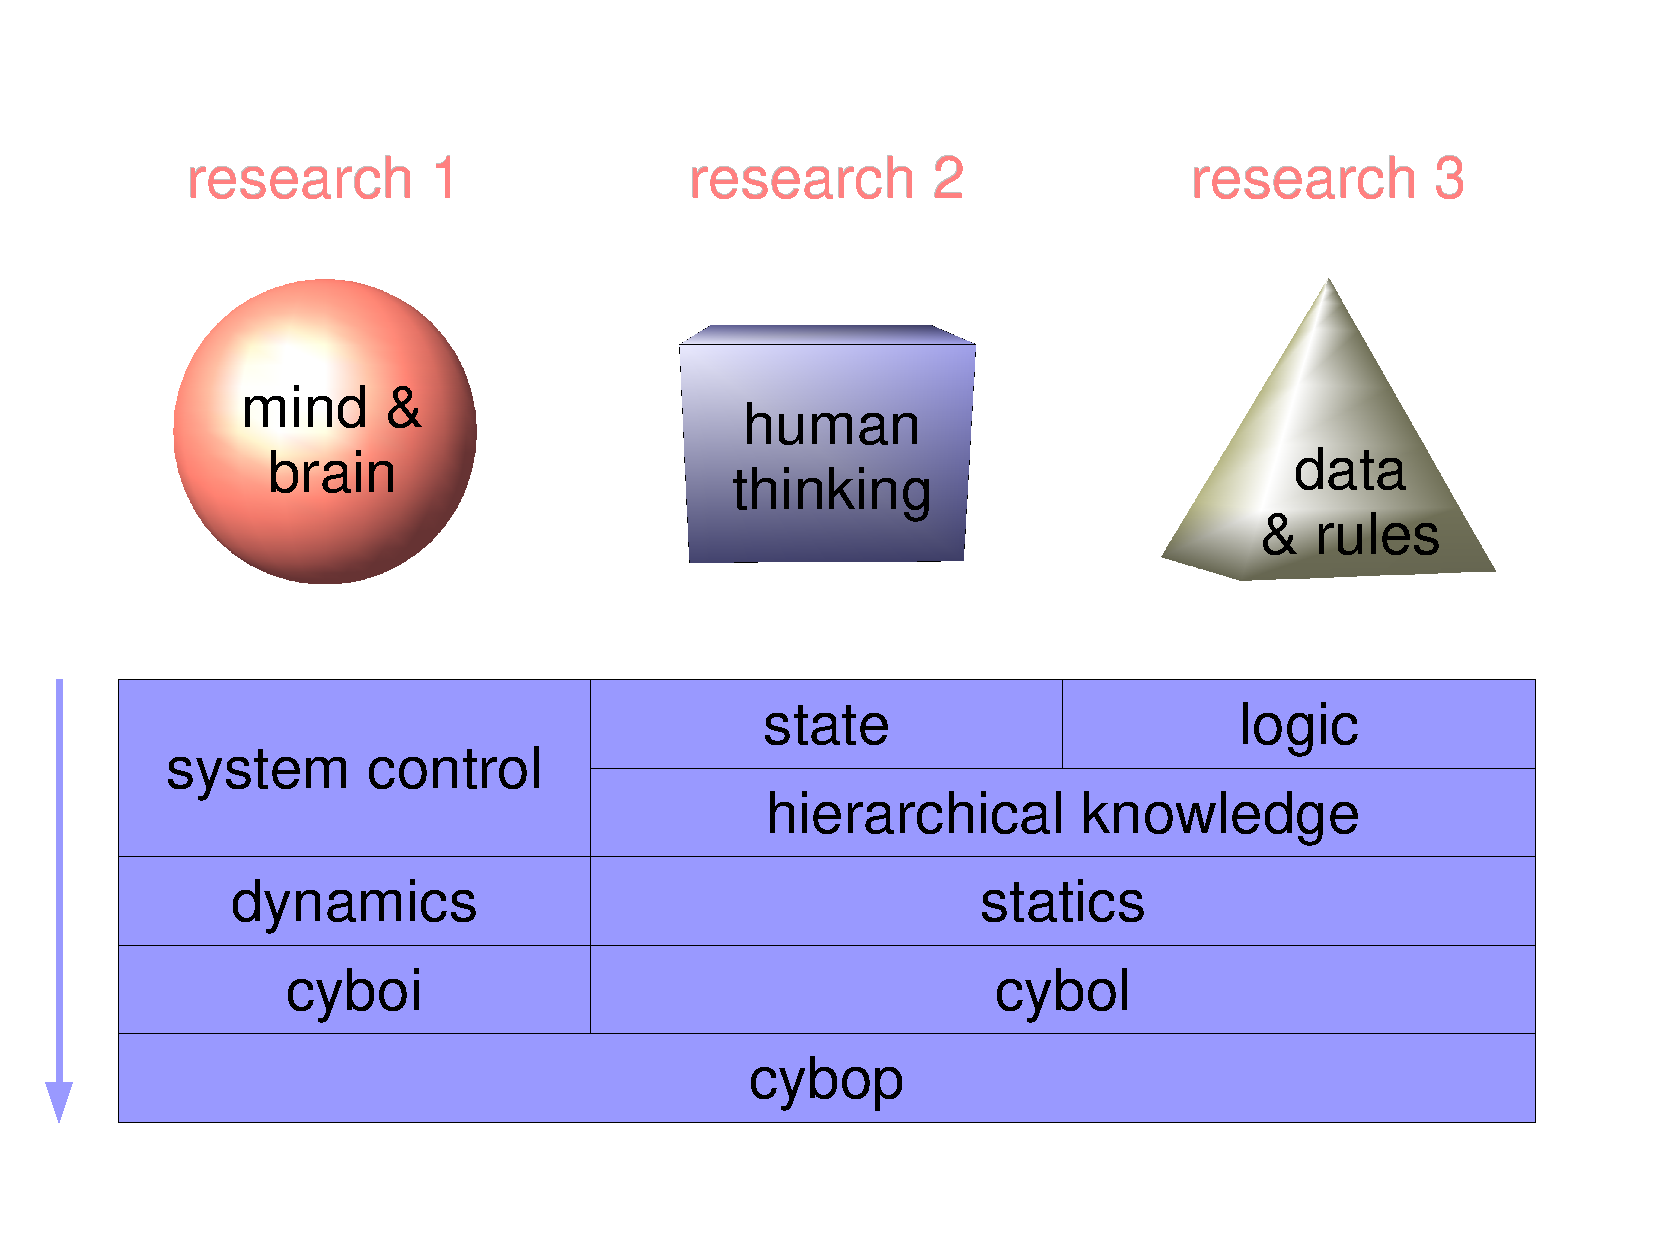
\includegraphics[scale=0.3,angle=-90]{graphic/approach.pdf}
        \caption{Overall CYBOP Approach Based on Statics and Dynamics}
        \label{cybop_approach_figure}
    \end{center}
\end{figure}

The complete modelling and storage of static knowledge requires a formal
language, which gets introduced as \emph{Cybernetics Oriented Language} (CYBOL)
in this work. Its dynamic processing, close to hardware, is guaranteed by the
\emph{Cybernetics Oriented Interpreter} (CYBOI) which is needed to run systems
defined in CYBOL (figure \ref{cybop_approach_figure}).

Chapters \ref{cybernetics_oriented_language_heading} and
\ref{cybernetics_oriented_interpreter_heading} explain CYBOL and CYBOI,
respectively. Both are used in the \emph{Res Medicinae} prototype application
which gets introduced in chapter \ref{res_medicinae_heading}. Altogether,
CYBOL, CYBOI and the theoretical concepts behind are called
\emph{Cybernetics Oriented Programming} (CYBOP).
